\documentclass[a4paper]{article}
\usepackage[letterpaper, margin=1in]{geometry} % page format
\usepackage{listings,graphicx,amsmath, amssymb, amsfonts, amsthm,tikz,hyperref,fullpage,setspace,enumerate,mathtools,arydshln}
\usepackage[english]{babel}

\title{Homework 4}
\author{Helen Ngo}
\date{\today}

\begin{document}
\lstset{language=Python,basicstyle=\ttfamily\footnotesize}

\maketitle

\begin {description}

\item[Problem 1] Use sklearn's implementation of $k$-Nearest Neighbors for regression purposes. Find the best value of $k$ using 10-fold Cross-Validation (CV).

\begin{enumerate}[(a)]
\item Generate 1000 data points.
\item Use 10-fold CV to report the three best values of $k$-neighbors that yield the best CV $E_{out}$; vary the values of $k$ in the following range: $k = 1, 3, 5, \dots, 2 \left \lfloor \frac{N+1}{2} \right \rfloor-1$.
\item Report the best CV $E_{out}$.
\end{enumerate}

\smallskip

\textbf{Solution:}
\begin{doublespace}
\begin{enumerate}[(a)]
\item The data was generated using the given genDataSet function, modified so that it only returned the input $x$ and target $y$ values. The ``Noisy Y" data was used as the target $y$ values:

\begin{center}
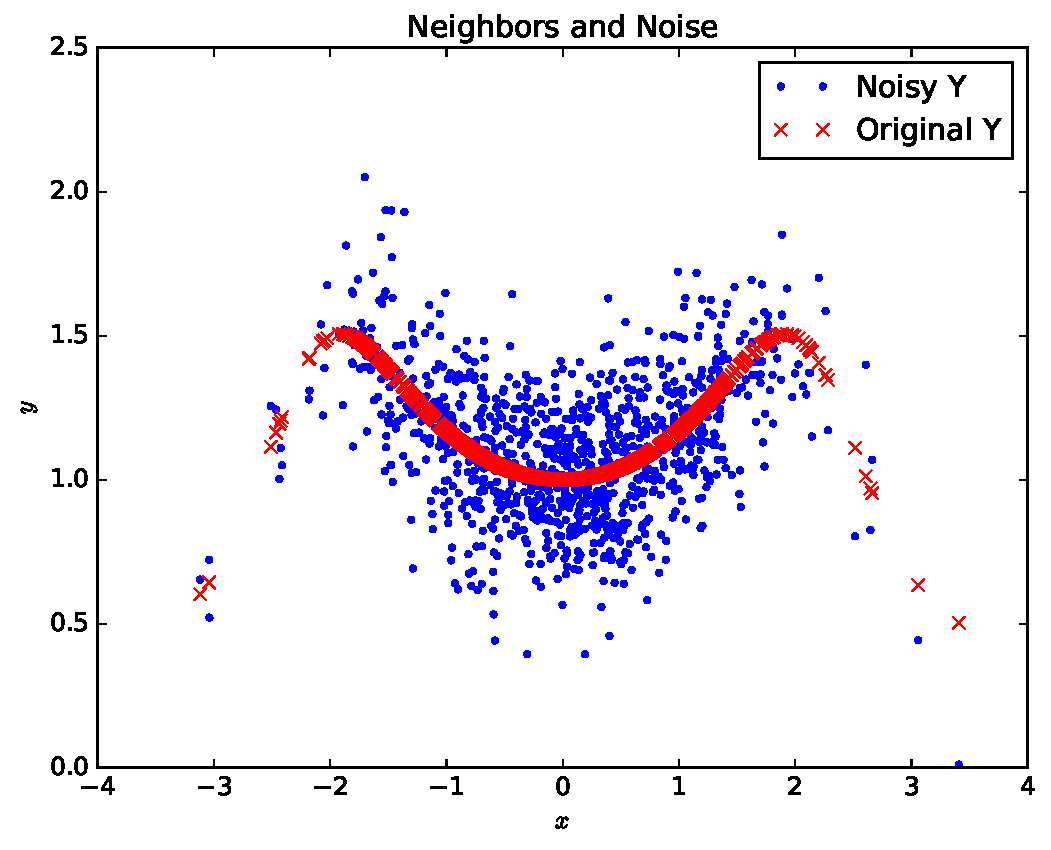
\includegraphics[scale=0.75]{neighbors.pdf}
\end{center}

This can be seen in the python document attached.
\item

\lstinputlisting[language=Python, firstline=28, lastline=49, frame=single]{neighbors.py}


Using the python code above, a list of $E_{out}$ for the given range of $k$ values was found. The index $i$ of the max value for the list of $E_{out}$ was determined, then used to calculate the corresponding $k$. Note that 

\begin{center}
\begin{tabular}{ c | c }
  k & index \\ \hline  
  1 & 0 \\
  3 & 1 \\
  5 & 2 \\
  \vdots & \vdots \\
  $2 \left \lfloor \frac{N+1}{2} \right \rfloor-1$& $\frac{k-1}{2}$ \\
\end{tabular},
\end{center}

therefore the $k$ value can be found from the index using the formula
\[k = 2(i) +1.\]

The index of the three best values of $k$-neighbors that yield the best CV $E_{out}$ were found: $k = 289, 296 $ and $303$. \footnote{Read footnote(2), these $k$ values were properly adjusted.}

\item The best CV $E_{out} = 0.245024051068$ was given by $k = 289$.
\end{enumerate}
\end{doublespace}

\item[Problem 2] Generate the dataset in the same way as in Problem 1. Repeat the experiment 100 times storing the best three $k$ number of neighbors in every single trial, and at the end of all the trials plot a histogram of all the saved values.

\smallskip

\textbf{Solution:}
\begin{doublespace}
Commenting out the plotting feature of the genDataSet function, the experiment was repeated a 100 times.
\lstinputlisting[language=Python, firstline=52, lastline=72, frame=single]{neighbors.py}

\newpage 

The following histogram was generated using the best $k$ values. \footnote{The $k$ number of neighbors may be 1 to 2 $k$ values off due to method of finding them, but this will do for examining the trend, such as for a histogram.}
\begin{center}
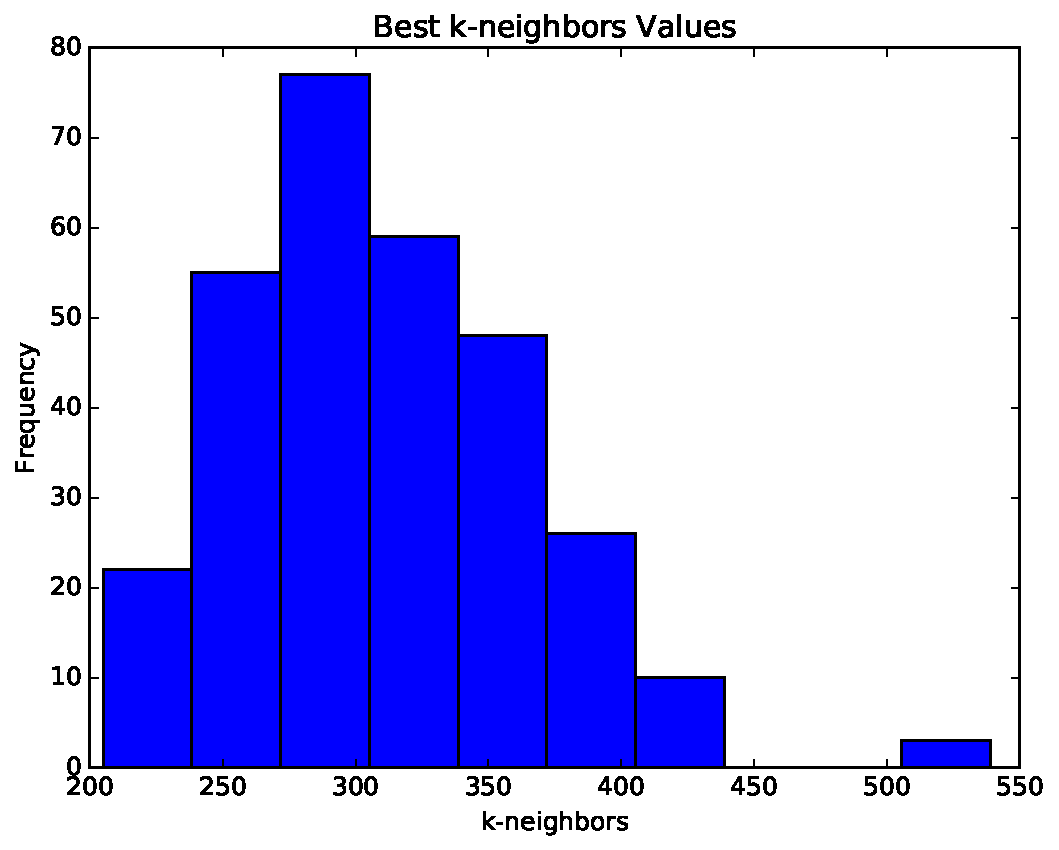
\includegraphics[scale=0.75]{khistogram.pdf}
\end{center}


\end{doublespace}

\end {description}
\end{document}
